\documentclass[dvipdfm]{beamer}
\usepackage{amsmath}
\usepackage{bm}
\usepackage{graphicx}
\usepackage{hyperref}
\usepackage{url}

%%ナビゲーションシンボルを表示しない
%%dvipdfmでは動かないため
\setbeamertemplate{navigation symbols}{}

\renewcommand{\kanjifamilydefault}{\gtdefault} % 和文既定をゴシックに変更

\title{PRML\_titech 2.3.1 - 2.3.7}
\author{榊原隆文(@saka\_bar)}
\date{November 21, 2014}

\setbeamertemplate{footline}[frame number]
\setbeamerfont{footline}{size=\small,series=\bfseries}
\setbeamercolor{footline}{fg=black,bg=black}

%数式をTeXの元々のフォントにする
\usefonttheme{professionalfonts}

\begin{document}
\maketitle

 \section*{自己紹介}
 \begin{frame}{自己紹介}
\begin{tabular}[tb]{cc}

 \begin{minipage}{0.5\hsize}
 \begin{center}
 \begin{itemize}
	\item さかばー(@saka\_bar)
	\item すずかけ台の奥村研に所属
				\begin{itemize}
				 \item 専門は自然言語処理
				 \item 知識獲得に興味あり
				\end{itemize}
	\item 好きなもの
				\begin{itemize}
				 \item 凌駕
				 \item 唐揚げ
				 \item Haskell
				 \item IIDX DP
				\end{itemize}
			 \end{itemize}
 \end{center}
 \end{minipage}

 \begin{minipage}{0.5\hsize}
 \begin{center}
 			 \begin{figure}[htbp]
				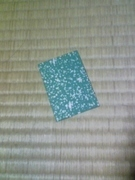
\includegraphics[bb=0 0 135 180,width=4.05cm,height=5.40cm]{./figure/icon.jpg}
				 \end{figure}
 \end{center}
 \end{minipage}
\end{tabular}



\end{frame}


 \begin{frame}{もくじ}
  \tableofcontents
 \end{frame}

 \section{2.3.1 条件付きガウス分布}
 \begin{frame}{2.3.1節と2.3.2節の目的}
 \begin{itemize}
  % \item 2つの変数集合の同時分布$p(x_a,x_b)$がガウス分布に従うなら、一方の変数集合が与えられたときの、もう一方の集合の条件付き分布$p(x_a|x_b)$もガウス分布になる
  \item 2つの変数集合の同時分布$p(x_a,x_b)$がガウス分布に従うときの、ガウス分布に関する以下の性質を示す
 \end{itemize}
 \begin{enumerate}
  \item 条件付き分布$p(x_a|x_b),p(x_b|x_a)$もガウス分布になる
  \item 変数集合の周辺分布$p(x_a),p(x_b)$もガウス分布になる
 \end{enumerate}
\end{frame}

\begin{frame}{変数の定義}
 \begin{itemize}
  \item 多変量ガウス分布の条件付き分布を考える
        \begin{equation}
         x\sim N(x|\mu, \Sigma)
        \end{equation}
        「$\sim$」はある分布に従う、ということ
  \item この$D$次元ベクトル$x$を2つの互いに素な部分集合$x_a$と$x_b$に分割する
  \item 次式のように、$x_a$は$x$の最初の$M$個の要素で、$x_b$は残りの$D-M$個の要素で構成されるとしても一般性は失わない
        \begin{equation}
         x =
          \begin{pmatrix}
           x_a \\
           x_b
          \end{pmatrix}
        \end{equation}

        \begin{equation}
         \mu =
          \begin{pmatrix}
           \mu_a \\
           \mu_b
          \end{pmatrix}
        \end{equation}
  \item 共分散行列も同様に与えられる
        \begin{equation}
         \Sigma =
          \begin{pmatrix}
           \Sigma_{aa} & \Sigma_{ab} \\
           \Sigma_{ba} & \Sigma_{bb}
          \end{pmatrix}
        \end{equation}
 \end{itemize}
\end{frame}

\begin{frame}{精度行列}
 \begin{itemize}
  \item \alert{精度行列}$\Lambda$を導入する
        \begin{equation}
         \Lambda \equiv \Sigma^{-1}
        \end{equation}

  \item ベクトル$x$の分割に対応する、分割された形式の精度行列を導入する
        \begin{equation}
         \Lambda=
          \begin{pmatrix}
           \Lambda_{aa} && \Lambda_{ab}\\
           \Lambda_{ba} && \Lambda_{bb}
          \end{pmatrix}
        \end{equation}
 \end{itemize}
\end{frame}


\begin{frame}{条件付きガウス分布}
 \begin{itemize}
  \item 条件付きガウス分布$p(x_a|x_b)$もガウス分布に従うことを示す
  \item 条件付きガウス分布は、次式のとおりである
        \begin{equation}
         p(x_a | x_b) = \frac{p(x_a, x_b)}{p(x_b)}
        \end{equation}
        \begin{itemize}
         \item $x_b$を観測済の値で\alert{固定}する
         \item 正規化係数を求めるのは後回し
        \end{itemize}
  % \item まず$p(x_a,x_b)$の指数部に注目する
  \item まずガウス分布の同時分布$p(x_a,x_b)$の指数部に注目する
 \end{itemize}
 \begin{equation}
  p(x_a,x_b) \sim N(x|\mu,\Sigma) = \frac{1}{(2\pi)^{D/2}}\frac{1}{|\Sigma|^{1/2}}exp\left\{-\frac{1}{2}(x - \mu)^{T}\Sigma^{-1}(x-\mu)\right\}
 \end{equation}
\end{frame}

\begin{frame}{条件付き分布の表現}
 \begin{itemize}
  \item ガウス分布の指数部分を展開する
        \begin{eqnarray}
         -\frac{1}{2}(x - \mu)^{T}\Sigma^{-1}(x-\mu) &= &
          -\frac{1}{2}(x_a - \mu_a)^{T}\Lambda_{aa}^{-1}(x_a-\mu_a) \nonumber \\
         &&-\frac{1}{2}(x_a - \mu_a)^{T}\Lambda_{ab}^{-1}(x_b-\mu_b) \nonumber \\
         &&-\frac{1}{2}(x_b - \mu_b)^{T}\Lambda_{ba}^{-1}(x_a-\mu_a) \nonumber \\
         &&-\frac{1}{2}(x_b - \mu_b)^{T}\Lambda_{bb}^{-1}(x_b-\mu_b) \nonumber \\
         &&\label{003314_21Nov14}
        \end{eqnarray}
  \item $x_a$の関数として見ると、これも\alert{二次形式}になっている
  % \item 対応する条件付き分布$p(x_a | x_b)$もガウス分布となる
 \end{itemize}
\end{frame}

\begin{frame}{平方完成}
 \begin{itemize}
		\item うまく変数$\mu_{a|b},\Sigma_{a|b}$を定めると、式(\ref{003314_21Nov14})の右辺は、式(\ref{135015_17Nov14})の右辺の形にすることができる
	\item 式(\ref{003314_21Nov14})の左辺の形に直すことで、ガウス分布の指数部の形にする
        \begin{equation}
         -\frac{1}{2}(x_a-\mu_{a|b})^{T}\Sigma_{a|b}^{-1}(x_a-\mu_{a|b}) = -\frac{1}{2}x_a^T\Sigma_{a|b}^{-1}x_a+x_a^T\Sigma_{a|b}^{-1}\mu_{a|b} + const\label{135015_17Nov14}
        \end{equation}
  \item 式(\ref{135015_17Nov14})の右辺から左辺への変形を\alert{平方完成}と呼ぶ

  % \item 平方完成したい式を式(\ref{135015_17Nov14})の右辺の形式で表現する
  % \item 式(\ref{135015_17Nov14})の右辺のように表現した式を左辺の形式に直す
  \item 与えられたガウス分布中の指数項を定める二次形式を平方完成するためには、分布の平均と分散を求める必要がある
  \item $x$の2次の項と1次の項の係数を比較することで、$\Sigma$と$\mu$を求めることができる
 \end{itemize}
\end{frame}

\begin{frame}{条件付きガウス分布の分散}
 \begin{itemize}
  \item 考えている条件付き分布はガウス分布に従うので、
        \begin{equation}
         p(x_a | x_b) \sim N(x | \mu_{a|b}, \Sigma_{a|b})
        \end{equation}
        と表せる
  \item まずは分散$\Sigma_{a|b}$を求める
  \item $x_b$を定数とみなして、式(\ref{003314_21Nov14})から$x_a$についての2次の項を全て取り出すと、
        \begin{equation}
         -\frac{1}{2}x_a^T\Lambda_{aa}x_a
        \end{equation}
        を得る。これより、
        \begin{equation}
         \Sigma_{a|b} = \Lambda_{aa}
        \end{equation}
        が得られる
 \end{itemize}
\end{frame}

\begin{frame}{条件付きガウス分布の平均}
 \begin{itemize}
  \item 次に平均$\mu_{a|b}$を求める
  \item $x_a$についての線形の項をすべて考えると、
        \begin{equation}
         x_a^T\{ \Lambda_{aa}\mu_a-\Lambda_{ab}(x_b)-\mu_b\}
        \end{equation}
        を得る
  \item この式の$x_a$の係数は$\Sigma^{-1}_{a|b}\mu_{a|b}$と等しくなるので、
        \begin{eqnarray}
         \mu_{a|b} &=& \Sigma_{a|b}\{\Lambda_{aa}\mu_a-\Lambda_{ab}(x_b-\mu_b)\}\\
         &= & \mu_a - \Lambda_{aa}^{-1}\Lambda_{ab}(x_b-\mu_b)
        \end{eqnarray}
 \end{itemize}
\end{frame}

\begin{frame}{精度行列を使わないで求める}
 次の関係
 \begin{equation}
  \begin{pmatrix}
   \Sigma_{aa} & \Sigma_{ab}  \\
   \Sigma_{ba} & \Sigma_{bb}
  \end{pmatrix}^{-1}=
  \begin{pmatrix}
   \Lambda_{aa} & \Lambda_{ab}  \\
   \Lambda_{ba} & \Lambda_{bb}
  \end{pmatrix}
 \end{equation}
 に対して、分割された行列の逆行列に関する次の公式(演習2.24)を利用
 \begin{equation}
  \begin{pmatrix}
   A & B \\
   C & D
  \end{pmatrix}^{-1}
  =
  \begin{pmatrix}
   M & -MBD^{-1} \\
   -D^{-1}CM & D^{-1}+D^{-1}CMBD^{-1}
  \end{pmatrix}\label{053319_21Nov14}
 \end{equation}
 ただし、
 \begin{equation}
  M=(A-BD^{-1}C)^{-1}
 \end{equation}
 $M^{-1}$を$D$に関するシューア補行列と呼ぶ
\end{frame}

\begin{frame}{計算結果}
 \begin{itemize}
  \item $\Lambda_{aa}$と$\Lambda_{ab}$は次のようになる
        \begin{eqnarray}
         \Lambda_{aa}&=&(\Sigma_{aa}-\Sigma_{ab}\Sigma_{bb}^{-1}\Sigma_{ba})^{-1} \\
         \Lambda_{ab}&= &-(\Sigma_{aa}-\Sigma_{ab}\Sigma_{bb}^{-1}\Sigma_{ba})^{-1} \Sigma_{ab}\Sigma_{bb}^{-1}
        \end{eqnarray}
  \item これらを
        \begin{eqnarray}
         \Sigma_{a|b} &=& \Lambda_{aa} \\
         \mu_{a|b}  &= & \mu_a - \Lambda_{aa}^{-1}\Lambda_{ab}(x_b-\mu_b)
        \end{eqnarray}
        の右辺に代入して、精度行列を消去する
 \end{itemize}
\end{frame}

\begin{frame}{精度行列を利用した表現と利用しない表現の比較}
 \begin{itemize}
  \item 得られた2つの表現は次の通りである
        \begin{eqnarray*}
         \mu_{a|b} &=& \mu_a + \Sigma_{ab}\Sigma_{bb}^{-1}(x_b-\mu_b)\\
         &=& \mu_a-\Lambda_{aa}^{-1}\Lambda_{ab}(x_b-\mu_b)
        \end{eqnarray*}
        \begin{eqnarray*}
         \Sigma_{a|b} &=& \Sigma_{aa} - \Sigma_{ab}\Sigma_{bb}^{-1}\Sigma_{ba} \\
         & =& \Lambda_{aa}^{-1}
        \end{eqnarray*}
  \item 条件付き分布$p(x_a|x_b)$は分割された共分散行列よりも、分割された精度行列を使って表現する方が簡潔
 \end{itemize}
\end{frame}


 \section{2.3.2 周辺ガウス分布}
 \begin{frame}{2.3.2 周辺ガウス分布}
 \begin{itemize}
  \item 同時分布$p(x_a,x_b)$がガウス分布であれば、条件付き分布$p(x_a|x_b)$もガウス分布になることを示した。
  \item この周辺分布
        \begin{equation}
         p(x_a) = \int p(x_a,x_b)dx_b
        \end{equation}
        がガウス分布になることを示す
  \item ここでも同時分布の指数部分の二次形式に注目し、周辺分布$p(x_a)$の平均と共分散を特定することで効率的に計算できる
 \end{itemize}
\end{frame}


\begin{frame}{計算の流れ}
 \begin{itemize}
  % \item 指数部の$x_b$に関係した項を処理してから、積分を容易にするために平方完成する
  \item $x_b$に関係ない項を$C_2$とおき$x_b$に関係した項に注目
        \begin{eqnarray*}
         && \int p(x_a,x_b)dx_b \\
         &=& \int \frac{1}{C_1}exp\left\{(x_b-\mu_1)^T\Lambda(x_b-\mu_1)+C_2\right\}dx_b \\
         &=& \frac{1}{C_1}exp\{C_2\}\underline{\int exp\left\{(x_b-\mu_1)^T\Lambda(x_b-\mu_1)\right\}dx_b}
        \end{eqnarray*}
        \begin{itemize}
         \item 下線部はガウス分布の積分なので積分結果は正規化係数の逆数(積分結果を$C_3$とおく)
        \end{itemize}
        \begin{eqnarray*}
         &=&\frac{1}{C_1}exp\{C_2\}C_3 \\
         &=&\frac{1}{C_1}exp\{(x_a-\mu_2)^T\Lambda (x_a-\mu_2)+C_4\}C_3\\
         &=&\frac{C_3}{C_1}\underline{exp\{C_4\}exp\{(x_a-\mu_2)^T\Lambda (x_a-\mu_2)}\}
        \end{eqnarray*}
  \item 指数部がガウス分布の形になる
 \end{itemize}
\end{frame}


\begin{frame}{計算}
 \begin{itemize}
  \item 指数部の$x_b$に関係した項を処理してから、積分を容易にするために平方完成する
  \item $x_b$を含む項を取り出すと
        \begin{eqnarray*}
         && -\frac{1}{2}(x - \mu)^{T}\bm{\Sigma}^{-1}(x-\mu) \\
         &=&-\frac{1}{2}x^T_b\Lambda_{bb}x_b+x^T_bm \\
         &=& -\frac{1}{2}(x_b-\Lambda_{bb}^{-1}m)^T\Lambda_{bb}(x_b-\Lambda_{bb}^{-1}m) + \frac{1}{2}m^T\Lambda_{bb}^{-1}m
        \end{eqnarray*}
        ただし、
        \begin{equation*}
         m =  \Lambda_{bb}\mu_b - \Lambda_{ba}(x_a-\mu_a)
        \end{equation*}
 \end{itemize}
\end{frame}

\begin{frame}{$x_b$の指数部}
 \begin{itemize}
  \item 指数部の式は次のとおり
        \begin{equation}
         -\frac{1}{2}(x_b-\Lambda_{bb}^{-1}m)^T\Lambda_{bb}(x_b-\Lambda_{bb}^{-1}m) + \frac{1}{2}m^T\Lambda_{bb}^{-1}m
        \end{equation}
        \begin{itemize}
         \item 右辺第1項はガウス分布の標準的な二次形式
         \item 残りの項は$x_b$に依存しない
        \end{itemize}
  \item $x_b$に関係しない部分を無視して考え、後で正規化係数を求めてつじつまを合わせる
        % \begin{equation}
        %  \int exp(f(x)+c)dx = exp(c)\int exp(f(x))dx
          % \end{equation}
 \end{itemize}
\end{frame}


\begin{frame}{途中計算}
 \begin{itemize}
  \item この二次形式の指数を取り、$x_b$で積分する
        % $x_b$に依存する部分を取り出して積分する
        \begin{eqnarray}
         \int exp\left\{-\frac{1}{2}(x_b-\Lambda_{bb}^{-1}m)^T\Lambda_{bb}(x_b-\Lambda_{bb}^{-1}m)\right\}dx_b
        \end{eqnarray}
  \item この積分は正規化されていないガウス分布なので、正規化係数の逆数になる。
  \item ガウス分布の正規化係数は平均とは独立で、共分散行列のみに依存するため、この積分も共分散行列のみに依存する
  \item 残った$x_a$に関する項を変形する
 \end{itemize}
\end{frame}

\begin{frame}{結論}
 \begin{itemize}
  \item 周辺分布$p(x_a)$の平均と共分散は次のようになる
        \begin{eqnarray}
         \mathbb{E}[x_a] &=&  \mu_a\\
         cov[x_a]&=&\bm{\Sigma}_{aa}
        \end{eqnarray}
  \item 分割された共分散行列について簡潔に表現される
        \begin{itemize}
         \item 条件付き分布のときと対照的
        \end{itemize}
 \end{itemize}
\end{frame}


 \section{2.3.3 ガウス変数に対するベイズの定理}
 \begin{frame}{2.3.3 ガウス分布の周辺分布と条件付き分布}
 \begin{itemize}
  \item あるガウス周辺分布$p(x)$と、平均が$x$の線形関数で共分散は$x$と独立であるようなガウス条件付き分布$p(y|x)$が与えられたとする
  \item このとき、周辺分布$p(y)$と条件付き分布$p(x|y)$を求める問題を考える
        \begin{itemize}
         \item この問題は以後の章でよく現れるので、ここで一般的な結果を求めておく
        \end{itemize}
 \end{itemize}
\end{frame}

\begin{frame}{変数の定義}
 \begin{itemize}
  \item 周辺分布と条件付き分布を
        \begin{eqnarray}
         p(x) &=& N(x|\bm{\mu} , \bm{\Lambda}^{-1})\\
         p(y|x) &=& N(y|Ax+b, L^{-1})
        \end{eqnarray}
        とする。
  \item 最初に、$x$と$y$の同時分布の表現を見る
        \begin{equation}
         z = \begin{pmatrix}
              x \\
              y
             \end{pmatrix}
        \end{equation}
        とおく
 \end{itemize}
\end{frame}

\begin{frame}{同時分布の対数}
 \begin{itemize}
  \item そして、同時分布の対数を考える
  \begin{itemize}
   \item ここで対数を考えるのは、いちいち「指数に注目」という手間を省くためだと考えられる
  \end{itemize}
        \begin{eqnarray}
         \ln p(z) &=& \ln p(x) + \ln p(y|x) \nonumber \\
         &= & -\frac{1}{2}(x-\bm{\mu})^{\mathrm{T}}\bm{\Lambda}(x-\bm{\mu}) \nonumber \\
         &&-\frac{1}{2}(y-Ax-b)^{\mathrm{T}}L(y-Ax-b)+{\rm const}\label{052313_21Nov14}
        \end{eqnarray}
  \item このガウス分布の精度行列を求めるために、式(\ref{052313_21Nov14})の2次の項についても考察する
 \end{itemize}
\end{frame}

\begin{frame}{2次の項と精度行列}
 \begin{itemize}
  \item 2次の項は次のように書ける
        \begin{eqnarray}
         -\frac{1}{2}x^{\mathrm{T}}(\bm{\Lambda}+A^{\mathrm{T}}LA)x -\frac{1}{2}y^{\mathrm{T}}Ly+\frac{1}{2}y^{\mathrm{T}}LAx+\frac{1}{2}x^{\mathrm{T}}A^{\mathrm{T}}Ly \nonumber \\
         = -\frac{1}{2}
          \begin{pmatrix}
           x \\
           y
          \end{pmatrix}^{\mathrm{T}}
          \begin{pmatrix}
           \bm{\Lambda}+A^{\mathrm{T}}LA & -A^{\mathrm{T}}L\\
           -LA & L
          \end{pmatrix}
          \begin{pmatrix}
           x \\
           y
          \end{pmatrix}
          = -\frac{1}{2}z^{\mathrm{T}}Rz
        \end{eqnarray}
  \item よって、$z$上のガウス分布の精度行列は
        \begin{equation}
         R=
          \begin{pmatrix}
           \bm{\Lambda}+A^{\mathrm{T}}LA & -A^{\mathrm{T}}L\\
           -LA & L
          \end{pmatrix}
        \end{equation}
        になる
 \end{itemize}
\end{frame}

\begin{frame}{共分散行列}
 \begin{itemize}
  \item 共分散行列は、行列の逆行列に関する公式(\ref{053319_21Nov14})を適用して精度の逆行列を求めることで求られる(演習2.29)
        \begin{equation}
         {\rm cov}[z]=R^{-1}=
          \begin{pmatrix}
           \bm{\Lambda}^{-1} & \bm{\Lambda}^{-1}A^{\mathrm{T}} \\
           A\bm{\Lambda}^{-1} & L^{-1} + A\bm{\Lambda}^{-1}A^{\mathrm{T}}
          \end{pmatrix}\label{054122_21Nov14}
        \end{equation}
 \end{itemize}
\end{frame}

\begin{frame}{$z$上のガウス分布の平均}
 \begin{itemize}
  \item 同様に、$z$上のガウス分布の平均は、(\ref{052313_21Nov14})の線形の項を調べることで、
        \begin{equation}
         x^{\mathrm{T}}\bm{\Lambda}\bm{\mu}-x^{\mathrm{T}}A^{\mathrm{T}}Lb+y^{\mathrm{T}}Lb =
          \begin{pmatrix}
           x \\
           y
          \end{pmatrix}^{\mathrm{T}}
          \begin{pmatrix}
           \bm{\Lambda}\bm{\mu}-A^{\mathrm{T}}Lb \\
           Lb
          \end{pmatrix}
        \end{equation}
        で与えられる
  \item 多変量ガウス分布の二次形式部分を平方完成して得た以前の結果より、$z$の平均は
        \begin{equation}
         \mathbb{E}[z]=R^{-1}
          \begin{pmatrix}
           \bm{\Lambda}\bm{\mu}-A^{\mathrm{T}}Lb \\
           Lb
          \end{pmatrix}
        \end{equation}
        を得る。式(\ref{054122_21Nov14})より、
        \begin{equation}
         \mathbb{E}[z]=
          \begin{pmatrix}
           \bm{\mu} \\
           A\bm{\mu} + b
          \end{pmatrix}
        \end{equation}
        を得る(演習2.30)
 \end{itemize}
\end{frame}

\begin{frame}{$x$を周辺化した周辺分布$p(y)$}
 \begin{itemize}
  \item ガウス確率ベクトルの要素の部分集合上の周辺分布を、分割された共分散行列で表したときの結果を利用する
  \item 周辺分布$p(y)$の平均と共分散は
        \begin{eqnarray}
         \mathbb{E}[y] &= &A\bm{\mu} +b\\
         {\rm cov}[y] &=& L^{-1} + A\bm{\Lambda}^{-1}A^{\mathrm{T}}
        \end{eqnarray}
        で与えられることがわかる
 \end{itemize}
\end{frame}


\begin{frame}{条件付き分布$p(x|y)$}
 \begin{itemize}
  \item 同様に、以前の結果を利用する
        \begin{eqnarray}
         \mathbb{E}[x|y]& =& (\bm{\Lambda}+A^{\mathrm{T}}LA)^{-1}\{A^{\mathrm{T}}L(y-b)+\bm{\Lambda}\bm{\mu}\}\\
         {\rm cov}[x|y] &= & (\bm{\Lambda}+A^{\mathrm{T}}LA)^{-1}
        \end{eqnarray}
  \item この条件付き分布は、ベイズの定理の例としても見ることができる
        \begin{itemize}
         \item $p(x)$は$x$上の事前分布と解釈できる
         \item 変数$y$が観測されれば、条件付き分布$p(x|y)$を用いて、$x$上での事後分布を表せる
         \item また、周辺分布と条件付き分布を求めれば、同時確率$p(z)=p(x)p(y|x)$は$p(x|y)p(y)$の形でも表現できる
        \end{itemize}
 \end{itemize}

\end{frame}


 \section{2.3.4 ガウス分布の最尤推定}
 \begin{frame}{2.3.4 ガウス分布の最尤推定}
 \begin{itemize}
  \item  ある多変量ガウス分布から、観測値$\{\bm{x}_n\}$が独立に得られたと仮定したデータ集合
         \begin{equation}
          X=(\bm{x}_1,...,\bm{x}_n)^{\mathrm{T}}
         \end{equation}
         がある時その分布のパラメータは最尤推定法で推定できる
  \item 尤度関数は、
        \begin{eqnarray*}
         && \ln  p(X|\bm{\mu}, \bm{\Sigma}) \\
         &=& -\frac{ND}{2}\ln (2\pi)-\frac{N}{2}\ln |\bm{\Sigma}|-\frac{1}{2}\sum_{n=1}^{N}(\bm{x}_n-\bm{\mu})^{\mathrm{T}}\bm{\Sigma}^{-1}(\bm{x}_n-\bm{\mu})
        \end{eqnarray*}
  \item これを整理すると、尤度関数は次の2つの量によってのみ依存していることが分かる
        \begin{eqnarray}
         \sum_{n=1}^{N}\bm{x}_n, \ \ \  \sum_{n=1}^{N}\bm{x}_n\bm{x}_n^{\mathrm{T}}
        \end{eqnarray}
  \item これらをガウス分布の\alert{十分統計量}という
 \end{itemize}
\end{frame}

\begin{frame}{最尤推定解}
 \begin{itemize}
  \item 最尤推定解は次のとおり
        \begin{eqnarray}
         \bm{\mu}_{ML} &=& \frac{1}{N}\sum_{n=1}^{N}\bm{x}_n\\
         \bm{\Sigma}_{ML}&=&\frac{1}{N}\sum_{n=1}^{N}(\bm{x}_n-\bm{\mu}_{ML})(\bm{x}_n-\bm{\mu}_{ML})^{\mathrm{T}}
        \end{eqnarray}
 \end{itemize}
\end{frame}

\begin{frame}{最尤推定解の期待値}
 \begin{itemize}
  \item 真の分布の下での最尤推定解の期待値を評価すると、次の結果を得る(演習2.35)
        \begin{eqnarray}
         \mathbb{E}[\bm{\mu}_{ML}]&=&\bm{\mu}\\
         \mathbb{E}[\bm{\Sigma}_{ML}]&=&\frac{N-1}{N}\bm{\Sigma}
        \end{eqnarray}
        \begin{itemize}
         \item 平均についての最尤推定量の期待値は真の平均に等しい
         \item 共分散の最尤推定量の期待値は真の値より小さいが、これは別の推定量$\widetilde{\bm{\Sigma}}$
               \begin{equation}
                \widetilde{\bm{\Sigma}} = \frac{1}{N-1}\sum_{n=1}^{N}(\bm{x}_n-\bm{\mu}_{ML})(\bm{x}_n-\bm{\mu}_{ML})^{\mathrm{T}}
               \end{equation}
               を定義することで補正することができる
        \end{itemize}
 \end{itemize}
\end{frame}


 \section{2.3.5 逐次推定}
 \begin{frame}{2.3.5 逐次推定}
 \begin{itemize}
  \item 逐次的な方法では、データ点を一度に1つずつ処理しては、それを廃棄する
  \item オンラインな応用分野や、すべてのデータ点を一度に一括処理することが不可能な大規模データ集合を扱う場合に重要
  \item まずは、平均の最尤推定量$\bm{\mu}_{ML}$について考える
 \end{itemize}
\end{frame}

\begin{frame}{平均の最尤推定量の逐次推定}
 \begin{itemize}
  \item $\bm{\mu}_{ML}^{N}$を変形すると、次のようになる
        \begin{eqnarray}
         \bm{\mu}_{ML}^{(N)} &= &\frac{1}{N}\sum_{n=1}^{N}\bm{x}_n \nonumber \\
         & =& \frac{1}{N}\bm{x}_N+\frac{1}{N}\sum_{n=1}^{N-1}\bm{x}_n \nonumber \\
         & =& \frac{1}{N}\bm{x}_N + \frac{N-1}{N}\bm{\mu}_{ML}^{(N-1)}\nonumber \\
         & =& \bm{\mu}_{ML}^{(N-1)} +\frac{1}{N} (\bm{x}_N-\bm{\mu}_{ML}^{(N-1)})\label{162008_21Nov14}
        \end{eqnarray}
 \end{itemize}
\end{frame}

\begin{frame}{逐次推定}
 \begin{itemize}
  \item この結果は次のように分かりやすく解釈できる
        \begin{eqnarray}
         \bm{\mu}_{ML}^{(N)} &= &\frac{1}{N}\sum_{n=1}^{N}\bm{x}_n \\
         & =& \bm{\mu}_{ML}^{(N-1)} +\frac{1}{N} (\bm{x}_N-\bm{\mu}_{ML}^{(N-1)})
        \end{eqnarray}
  \item $N-1$個のデータを観測した時点で、$\bm{\mu}$の推定値は$\bm{\mu}_{ML}^{(N-1)}$となっている。
  \item ここで、データ点$\bm{x}_N$を観測すると、$1/N$に比例する小さな量だけ「誤差信号」$(\bm{x}_N-\bm{\mu}_{ML}^{(N-1)})$の方へ、古い推定量を移動させて推定量$\bm{\mu}_{ML}^{(N)}$を修正する
  \item Nが増えるにつれて、後続のデータ点からの影響はより小さくなる
 \end{itemize}
\end{frame}

\begin{frame}{汎用的な逐次学習の定式化}
 \begin{itemize}
  \item 先の例では、全体をまとめてバッチ処理する式と逐次推定する式が等しいので、明らかに同じ解が得られる
  \item しかしこの方法で逐次アルゴリズムを導出することが、いつもできるわけではない
  \item \alert{Robbins-Monroアルゴリズム}を導入する
 \end{itemize}
\end{frame}


%%TODO 図2.10の挿入
\begin{frame}{準備}
 \begin{itemize}
  \item 同時分布$p(z,\theta)$に従う確率変数$\theta$と$z$の対を考える
  \item $\theta$が与えられたときの$z$の条件付き期待値によって、決定論的な関数$f(\theta)$を定義する
        \begin{equation}
         f(\theta) \equiv \mathbb{E}[z|\theta] = \int zp(z|\theta)dz
        \end{equation}
        \begin{itemize}
         \item このように定義された関数を回帰関数と呼ぶ
        \end{itemize}
  \item ここでの目標は、$f(\theta^\ast)=0$の根$\theta^\ast$を求めること
 \end{itemize}
\end{frame}

\begin{frame}{仮定}
 \begin{itemize}
  \item 次のような仮定を置く
        \begin{eqnarray}
         \mathbb{E}[(z-f)^2|\theta] &<& \infty\\
         \theta^{(N)}&=& \theta^{(N-1)}-a_{N-1}z(\theta^{(N-1)})
        \end{eqnarray}
  \item ただし、$z(\theta^{(N)})$は$\theta$が値$\theta^{(N)}$を取るときに観測される$z$の値
  \item 係数$\{a_N\}$は以下の条件を満たす正数の系列
        \begin{equation}
         \lim_{N \rightarrow \infty}a_N=0
        \end{equation}
        \begin{itemize}
         \item この過程が極限値に収束できるように、解の逐次的な修正量を減らすことを保証
        \end{itemize}
        \begin{equation}
         \sum_{N=1}^{\infty}a_N=\infty
        \end{equation}
        \begin{itemize}
         \item アルゴリズムが根以外に速すぎる収束をしないことを保証
        \end{itemize}
        \begin{equation}
         \sum_{N=1}^{\infty}a_N^2 < \infty
        \end{equation}
        \begin{itemize}
         \item 蓄積されたノイズの分散を有限に抑え、収束を阻害しないことを保証
        \end{itemize}
 \end{itemize}
\end{frame}

%%TODO 大カッコを大きくする
\begin{frame}{Roobins-Monroアルゴリズム}
 \begin{itemize}
  \item 定義より、最尤推定解$\theta_{ML}$は負の対数尤度関数の停留点であるため、
        \begin{equation}
         -\frac{\partial }{\partial \theta}\left\{\left.\frac{1}{N}\sum_{n=1}^{N}\ln  p(\bm{x}_n|\theta)\right\}\right|_{\theta_{ML}} = 0
        \end{equation}
  \item 微分と総和の演算を交換し、$N\rightarrow\infty$の極限を考えると次の式を得る
        \begin{equation}
         -\lim_{N \rightarrow \infty}\frac{1}{N}\sum_{n=1}^{N}\frac{\partial}{\partial \theta}\ln p(\bm{x}_n|\theta)=\mathbb{E}_x\left[-\frac{\partial}{\partial \theta}\ln p(x|\theta)\right]
        \end{equation}
 \end{itemize}
\end{frame}

\begin{frame}{Robbins-Monro手続きの適用}
 \begin{itemize}
  \item 最尤推定解を求めることは、回帰関数の根を求めることに相当することがわかる
  \item ゆえに、次の形でRobbins-Monro手続きを適用できる
        \begin{equation}
         \theta^{(N)}=\theta^{(N-1)}-a_{N-1}\frac{\partial}{\partial \theta^{(N-1)}}[-\ln p(\bm{x}_N|\theta^{(N-1)})]\label{161911_21Nov14}
        \end{equation}
 \end{itemize}
\end{frame}

\begin{frame}{ガウス分布への適用}
 \begin{itemize}
  \item パラメータ$\theta^{(N)}$はガウス分布の平均の推定量$\bm{\mu}_{ML}^{(N)}$であり、確率変数$z$は
        \begin{equation}
         z=-\frac{\partial}{\partial \bm{\mu}_{ML}} \ln p(x|\bm{\mu}_{ML}, \sigma^2) = -\frac{1}{\sigma^2}(x-\bm{\mu}_{ML})\label{161904_21Nov14}
        \end{equation}
  \item 式(\ref{161904_21Nov14})を式(\ref{161911_21Nov14})に代入し、係数$a_N$を$a_N=\sigma^2/N$となるように選ぶと、式(\ref{162008_21Nov14})の1変数の形式のものが得られる
 \end{itemize}
\end{frame}


 \section{2.3.6 ガウス分布に対するベイズ推論}
 \begin{frame}{2.3.6 ガウス分布に対するベイズ推論}
 \begin{itemize}
  \item 今までは最尤推定の枠組みのガウス分布パラメータ$\mu$と$\bm{\Sigma}$の点推定量を得た
  \item 次に、事前分布を導入してベイズ主義的に扱う
        \begin{itemize}
         \item 分散が既知のとき
         \item 平均が既知のとき
         \item 平均も分散も未知のとき
        \end{itemize}
 \end{itemize}
\end{frame}

\begin{frame}{分散が既知のときの事前分布}
 \begin{itemize}
  \item \alert{分散$\sigma^2$は既知}とし、与えられた$N$個の観測値集合$x=\{x_1,...,x_N\}$から、平均$\mu$を推定する
  \item $\mu$が与えられたときに観測データが生じる確率である尤度関数は$\mu$の関数と見なせて、
        \begin{eqnarray*}
         p(X|\mu) &= &\prod_{n=1}^{N}p(x_n|\mu) \\
         &=& \frac{1}{(2\pi\sigma^2)^{N/2}}\exp\left\{-\frac{1}{2\sigma^2}\sum_{n=1}^{N}(x_n-\mu)^2\right\}
        \end{eqnarray*}
  % \item ただし、尤度関数は$\mu$上の確率分布ではなく、正規化もされていない
  \item 尤度関数を見ると、$\mu$についての二次形式の指数の形を取っている
  \item 前事分布$p(\mu)$にガウス分布を選べば、この尤度関数の共役事前分布となる
 \end{itemize}
\end{frame}

\begin{frame}{共役事前分布}
 \begin{itemize}

  \item 事前分布を次のようにする
        \begin{equation}
         p(\mu) = N(\mu|\mu_0,\sigma_0^2)
        \end{equation}
  \item すると事後分布は
        \begin{equation}
         p(\mu|X) \propto p(X|\mu)p(\mu)w
        \end{equation}
        となる
 \end{itemize}
\end{frame}

\begin{frame}{事後分布の平均と分散}
 \begin{itemize}
  \item 事後分布の指数部分は、
        \begin{eqnarray}
         & &\exp\left\{-\frac{1}{2\sigma_0^2}(\mu-\mu_0)^2\right\} \exp\left\{-\frac{1}{2\sigma^2}\sum_{n=1}^{N}(\mu-x_n)^2\right\} \nonumber \\
         &= & \exp\left\{-\frac{1}{2}\left(\frac{1}{\sigma_0^2}+\frac{N}{\sigma^2}\right)\mu^2 +\left(\frac{\mu_0}{\sigma_0^2}+\frac{1}{\sigma^2}\sum_{n=1}^{N}x_n\right)\mu +C_0 \right\} \nonumber
        \end{eqnarray}
  \item 平方完成と正規化によって平均$\mu_N$,分布$\sigma_N^2$のガウス分布の形にすることができる。ただし、
        \begin{eqnarray}
         \mu_N& = & \frac{\sigma^2}{N\sigma_0^2+\sigma^2}\mu_0 + \frac{N\sigma_0^2}{N\sigma_0^2+\sigma^2}\mu_{ML}\label{223654_18Nov14}\\
         \frac{1}{\sigma_N^2}&= & \frac{1}{\sigma_0^2} + \frac{N}{\sigma^2}\label{181817_24Nov14}\\
         \mu_{ML}&= & \frac{1}{N}\sum_{n=1}^{N}x_n
        \end{eqnarray}
 \end{itemize}
\end{frame}

\begin{frame}{平均と分散の性質}
 \begin{eqnarray}
  \mu_N& = & \frac{\sigma^2}{N\sigma_0^2+\sigma^2}\mu_0 + \frac{N\sigma_0^2}{N\sigma_0^2+\sigma^2}\mu_{ML}\label{181902_24Nov14}\\
  \frac{1}{\sigma_N^2}&= & \frac{1}{\sigma_0^2} + \frac{N}{\sigma^2}
 \end{eqnarray}
 \begin{itemize}
  \item $N\rightarrow0$なら、予想通り式(\ref{181902_24Nov14})は事前分布の平均
  \item $N\rightarrow\infty$なら、事後分布の最尤推定解となる
  \item $N\rightarrow0$なら、事前分布の分散に一致
  \item $N\rightarrow\infty$なら、分散は最尤推定解に一致
 \end{itemize}
\end{frame}

\begin{frame}{ここまで書いた}
 \begin{itemize}
  \item がんばろう。
 \end{itemize}
\end{frame}

\begin{frame}{事後分布のもう一つの見方}
 \begin{itemize}
  \item $N$個のデータ点を観測した後の平均は、$N$番目のデータ点$x_N$の影響と$N-1$個のデータ点を観測した後の平均とでも表現できた
  \item このことをガウス分布の平均の推論の場合について示す
        \begin{equation}
         p(\mu|X) \propto \left[p(\mu)\prod_{n=1}^{N-1}p(x_n|\mu)\right]p(x_N|\mu)
        \end{equation}
  \item カギカッコ内の項は正規化係数を除いて、$N-1$個のデータ点を観測した後の事後分布にちょうど一致する
  \item この項を事前分布とし、データ点$x_N$についての尤度関数をベイズの定理によって結合すれば、この式全体は$N$個のータ点を観測した後の事後分布とみなせる
 \end{itemize}
\end{frame}

\begin{frame}{平均が既知の場合}
 \begin{itemize}
  % \item \alert{平均が既知}の場合、事前分布に共役な分布を選ぶと計算が単純化
  \item 精度$\lambda\equiv 1/\sigma^2$で操作
        \begin{eqnarray}
         p(X|\lambda) &=& \prod_{n=1}^{N}N(x_n|\mu,\lambda^{-1}) \nonumber \\
         &=& \lambda^{N/2}\exp\left\{-\frac{\lambda}{2}\sum_{n=1}^{N}(x_n-\mu)^2\right\}\label{114403_19Nov14}
        \end{eqnarray}
  \item この式から、精度の共役事前分布は、$\lambda$のベキ乗と、$\lambda$の線形関数の指数の積に比例させる
        \begin{itemize}
         \item \alert{ガンマ分布}
        \end{itemize}
 \end{itemize}
\end{frame}


\begin{frame}{ガンマ分布}
 \begin{itemize}
  \item ガンマ分布の定義
        \begin{equation}
         Gam(\lambda|a,b) = \frac{1}{\Gamma(a)}b^a\lambda^{a-1}\exp(-b\lambda)\label{113739_19Nov14}
        \end{equation}
  \item ここで、$\Gamma(a)$は式(\ref{113739_19Nov14})が正しく正規化されることを保証
        %% TODO ガンマ関数の図を入れる
  \item ガンマ関数の平均と分散は
        \begin{eqnarray}
         \mathbb{E}[\lambda] &=& \frac{a}{b}\\
         var[\lambda]& =& \frac{a}{b^2}
        \end{eqnarray}
 \end{itemize}
\end{frame}

\begin{frame}{事前分布}
 \begin{itemize}
  \item 事前分布$Gam(\lambda|a_0,b_0)$について考える
  \item これに尤度関数(\ref{114403_19Nov14})をかけると、事後分布
        \begin{equation}
         p(\lambda|X) \propto \lambda^{a_0-1}\lambda^{N/2}\exp\left\{-b_0\lambda-\frac{\lambda}{2}\sum_{n=1}^{N}(x_n-\mu)^2\right\}\label{114734_19Nov14}
        \end{equation}
        が得られる
  \item これはパラメータを次のように設定したときの、ガンマ分布$Gam(\lambda|a_N,b_N)$であることが分かる
        \begin{eqnarray}
         a_N&=& a_0 + \frac{N}{2}`\label{115004_19Nov14}\\
         b_N% &= & b_0+\frac{1}{2}\sum_{n=1}^{N}(x_n-\mu)^2\\
         &= & b_0+\frac{N}{2}\sigma^2_{ML}\label{115046_19Nov14}
        \end{eqnarray}
 \end{itemize}
\end{frame}

\begin{frame}{パラメータの性質(非表示?)}
 \begin{itemize}
  \item 式(\ref{114734_19Nov14})では、事前分布や尤度関数で正規化係数を維持更新する必要はない
        \begin{itemize}
         \item 必要に応じて、正規化されたガンマ分布(\ref{113739_19Nov14})を用いて正しい係数を求めることができるため
        \end{itemize}
  \item 式(\ref{115004_19Nov14})より、$N$個のデータ点を観測すると、係数$a$を$N/2$だけ増やす効果がある
        \begin{itemize}
         \item 事前分布のパラメータ$a_0$は、$2a_0$個の「有効な」観測値が事前にあると解釈できる
        \end{itemize}
  \item 式(\ref{115046_19Nov14})より、$N$個のデータ点は$N\sigma_{ML}^2/2$だけ、パラメータ$b$に影響を及ぼす
        \begin{itemize}
         \item 事前分布のパラメータ$b_0$は、その分布が$b_0/a_0$であるような、$2a_0$個の「有効な」観測値が事前にあると解釈できる
        \end{itemize}
 \end{itemize}
\end{frame}

\begin{frame}{逆ガンマ分布}
 \begin{itemize}
  \item 精度について考える代わりに、分散そのものについて考えることもできる
  \item 逆ガンマ分布
        \begin{itemize}
         \item ここでは触れない
        \end{itemize}
 \end{itemize}
\end{frame}

\begin{frame}{平均と分散が未知の場合}
 \begin{itemize}
  \item \alert{平均と分散が未知}の場合には、共役事前分布を求めるために尤度関数の$\mu$と$\lambda$への依存関係について考える
        \begin{eqnarray}
         p(X|\mu,\lambda) &=& \prod_{n=1}^{N}(\frac{\lambda}{2\pi})^{1/2}\exp\{-\frac{\lambda}{2}(x_n-\mu)^2\} \nonumber \\
         &\propto & [\lambda^{1/2}\exp(-\frac{\lambda\mu^2}{2})]^{N}\exp\{\lambda\mu\sum_{n=1}^{N}x_n-\frac{\lambda}{2}\sum_{n=1}^{N}x_n^2\}
        \end{eqnarray}
 \end{itemize}
\end{frame}

\begin{frame}{事前分布}
 \begin{itemize}
  \item ここでは、尤度関数と同じ$\mu$と$\lambda$への関数依存性を備えた事前分布$p(\mu,\lambda)$を求めたいので、分布は次の形式になる
        \begin{eqnarray}
         p(\mu,\lambda) &\propto& [\lambda^{1/2}\exp(-\frac{\lambda\mu^2}{2})]^\beta \exp\{c\lambda\mu-d\lambda\} \nonumber \\
         &= & \exp\{-\frac{\beta\lambda}{2}(\mu-c\beta)^2\}\lambda^{\beta/2}\exp\{-(d-\frac{c^2}{2\beta})\lambda\}
        \end{eqnarray}
  \item 常に$p(\mu,\lambda)=p(\mu|\lambda)p(\lambda)$と書けるので、$p(\mu|\lambda)$と$p(\lambda)$に対応する部分を見出せばよい
  \item $p(\mu|\lambda)$は精度が$\lambda$の線形関数であるガウス分布であり、$p(\lambda)$はガンマ分布であることがわかる
  \item よって、定数$\mu_0=c/\beta, a=(1+\beta)/2,$および$b=d-c^2/2\beta$を新たに定義すると、正規化した事前分布は次の形を取る
        \begin{equation}
         p(\mu,\lambda)=N(\mu|\mu_0, (\beta\lambda)^{-1})Gam(\lambda|a,b)
        \end{equation}
  \item この分布を\alert{正規-ガンマ分布}や\alert{ガウス-ガンマ分布}と呼ぶ
 \end{itemize}
\end{frame}

\begin{frame}{正規-ガンマ分布の特徴}
 \begin{itemize}
  \item この分布は、独立な$\mu$上のガウス事前分布と$\lambda$上のガンマ事前分布の単純な積ではない
        \begin{itemize}
         \item $\mu$の分布の精度は$\lambda$の線形関数になっているため
        \end{itemize}
  \item たとえ$\mu$と$\lambda$が独立な事前分布を選んでも、事後分布では$\mu$の分布の精度と$\lambda$との間に関連が生じる
 \end{itemize}
\end{frame}

\begin{frame}{ウィシャート分布}
 \begin{itemize}
  \item $D$次元変数の多変量ガウス分布の場合に、\alert{精度を既知}とすれば、平均$\mu$の共役事前分布は、またガウス分布になる
  \item \alert{平均が既知}で、精度行列$\bm{\Lambda}$が未知なら、共役事前分布は次式のウィシャート分布となる
        \begin{equation}
         W(\bm{\Lambda}|W,\nu) = B|\bm{\Lambda}|^{(\nu-D-1)/2}\exp\left(-\frac{1}{2}Tr(W^{-1}\bm{\Lambda})\right)
        \end{equation}
        % \begin{itemize}
  %  \item $\nu$は分布の自由度パラメータ
  %  \item $W$は$D \times D$の尺度行列
  %  \item $Tr($・$)$はトレース
  %  \item $B$は次式
          % \end{itemize}
        \begin{equation}
         B(W,\nu) = |W|^{-\nu/2}\left(2^{\nu D/2}\pi^{D(D-1)/4}\prod_{i=1}^D\Gamma\left(\frac{\nu+1-i}{2}\right)\right)^{-1}
        \end{equation}
  \item ここでも、精度行列上ではなく、共分散行列上の共役事前分布を定義できる
        \begin{itemize}
         \item 逆ウィシャート分布(ここでは触れない)
        \end{itemize}
 \end{itemize}
\end{frame}

\begin{frame}{正規-ウィシャート分布}
 \begin{itemize}
  \item \alert{平均と精度の両方が未知}なら、1変数の場合と同様に考えることで次の共役事前分布が得られる
        \begin{equation}
         p(\mu,\bm{\Lambda}|\mu_0,\beta,W,\nu) = N(\mu|\mu_0,(\beta\bm{\Lambda})^{-1})W(\lambda|W,\nu)
        \end{equation}
  \item \alert{正規-ウィシャート分布}または\alert{ガウス-ウィシャート分布}と呼ぶ
 \end{itemize}
\end{frame}


 \section{2.3.7 スチューデントのt分布}
 \begin{frame}{2.3.7 スチューデントのt分布}
 \begin{itemize}
  \item これまでに、ガウス分布の精度パラメータの共役事前分布がガンマ分布となることを見てきた
  \item 1変数のガウス分布$\mathcal{N}(x|\mu, \tau^{-[bb=0 0 817 592]1})$において、ガンマ分布${\rm Gam}(\tau|a,b)$を精度の事前分布とし、そこから精度を積分消去し、$z=\tau[b+(x-\mu)^2/2]$の変数の置換を用いると、$x$の周辺分布は次式となる
        \begin{eqnarray}
         && p(x|\mu,a,b) \nonumber \\
         &=& \int_0^\infty \mathcal{N}(x|\mu,\tau^{-1}){\rm Gam}(\tau|a,b)d\tau\label{133939_19Nov14} \\
         % &= & \int_{0}^{\infty}\frac{b^ae^{-b\tau}\tau^{a-1}}{\Gamma(a)}(\frac{\tau}{2\pi})^{1/2}\exp\{-\frac{\tau}{2}(x-\mu)^2\}d\tau \nonumber\\
         &= & \frac{b^a}{\Gamma(a)}\left(\frac{1}{2\pi}\right)^{1/2}\left[b+\frac{(x-\mu)^2}{2}\right]^{-a-1/2}\!\!\!\!\!\!\Gamma(a+1/2)
        \end{eqnarray}
 \end{itemize}
\end{frame}

\begin{frame}{スチューデントのt分布}
 \begin{itemize}
  \item 慣例により、$\nu=2a$と$\lambda=a/b$のパラメータを新たに定義すると、\alert{スチューデントのt分布}が得られる
        \begin{equation}
         {\rm St}(x|\mu,\lambda,\nu) = \frac{\Gamma(\nu/2+1/2)}{\Gamma(\nu/2)}\left(\frac{\lambda}{\pi\nu}\right)^{1/2}\left[1+\frac{\lambda(x-\mu)^2}{\nu}\right]^{-\nu/2-1/2}
        \end{equation}
        \begin{itemize}
         \item パラメータ$\lambda$はt分布の精度とも呼ばれるが、必ずしも分散の逆数とは限らない
         \item パラメータ$\nu=1$ではコーシー分布、$\nu\rightarrow\infty$では平均が$\mu$で精度が$\lambda$のガウス分布になる
        \end{itemize}
  \item 式(\ref{133939_19Nov14})より、スチューデントのt分布は、平均は同じだが精度は異なるようなガウス分布を無限個足し合わせたものであることがわかる
        \begin{itemize}
         \item ガウス分布の無限混合分布(詳細は2.3.9節)
        \end{itemize}
 \end{itemize}
\end{frame}

%図を挿入するときは.epsファイルを使う
%jpgなどだと、画面外に画像が配置される(意味不明)
% .epsは神。
\begin{frame}{スチューデントのt分布}
 \begin{center}
  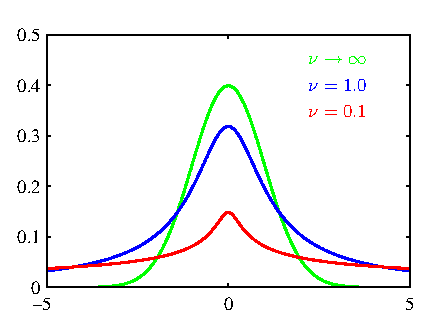
\includegraphics[scale=1.0]{./figure/Figure2.15.eps}
 \end{center}
\end{frame}

\begin{frame}{頑健性と回帰問題}
 \begin{itemize}
  \item スチューデントのt分布はガウス分布より一般に「すそ」が長く、\alert{頑健性}を持つ
        \begin{itemize}
         \item 外れ値となっている少数のデータ点があっても、ガウス分布よりは影響されにくい
        \end{itemize}
  % \item 外れ値は、実際にデータを生成する分布のすそが大きい場合や、単純なラベル付けの誤りなどにあるように、実際の問題ではよく生じる
  % \item 頑健性は回帰問題でも重要な性質である
  % \item 回帰での最小二乗法は、条件付きガウス分布の下での最尤推定に相当するので、頑健ではない
  % \item そこで、すその重い分布に基づく回帰モデルを用いる
 \end{itemize}
        \begin{tabular}[tb]{cc}
         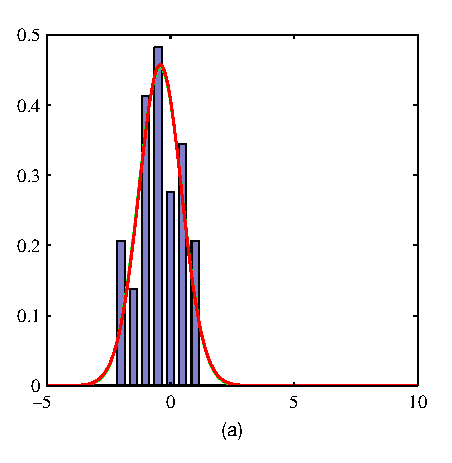
\includegraphics[width=0.5\textwidth]{./figure/Figure2.16a.eps}
         &
         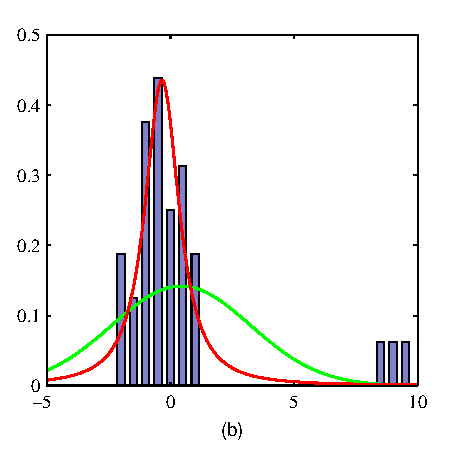
\includegraphics[width=0.5\textwidth]{./figure/Figure2.16b.eps}
        \end{tabular}
\end{frame}

\begin{frame}{多変量のスチューデントt分布}
 \begin{itemize}
  \item 式(\ref{133939_19Nov14})に戻って、パラメータを$\nu=2a,\lambda=a/b,$および$\eta=\tau b/a$と置き換えると、t分布は次の形に書ける
        \begin{equation}
         {\rm St}(x|\mu,\lambda,\nu) = \int_{0}^{\infty}\mathcal{N}(x|\mu, (\eta\lambda)^{-1}){\rm Gam}(\eta|\nu/2,\nu/2)d\eta
        \end{equation}
  \item これは多変量ガウス分布の場合に一般化でき、多変量スチューデントt分布に相当するものが次式で得られる
        \begin{equation}
         {\rm St}(\bm{x}|\bm{\mu},\bm{\Lambda},\nu) = \int_{0}^{\infty}\mathcal{N}(\bm{x}|\bm{\mu}, (\eta\bm{\Lambda})^{-1}){\rm Gam}(\eta|\nu/2,\nu/2)d\eta
        \end{equation}
 \end{itemize}
\end{frame}

\begin{frame}{多変量のスチューデントt分布}
 \begin{itemize}
  \item 1変数の場合と同じように、積分を計算すると
        \begin{eqnarray}
         {\rm St}(\bm{x}|\bm{\mu},\bm{\Lambda},\nu) &=& \frac{\Gamma(D/2+\nu/2)}{\Gamma(\nu/2)}\frac{|\bm{\Lambda}|^{1/2}}{(\pi\nu)^{D/2}}\left[1+\frac{\Delta^2}{\nu}\right]^{-D/2-\nu/2} \\
         \Delta^2&= & (\bm{x}-\bm{\mu})^{\mathrm{T}}\bm{\Lambda}(\bm{x}-\bm{\mu})
        \end{eqnarray}
        を得る
  \item これはスチューデントt分布の多変量型で、1変数の結果に対応した、次の性質を満たす
        \begin{align}
         \mathbb{E}[\bm{x}]&=& \bm{\mu}&, && \text{$\nu>1$のとき}\\
         {\rm cov}[\bm{x}]&=&\frac{\nu}{(\nu-2)}\bm{\Lambda}^{-1}&,  &&\text{$\nu>2$のとき}\\
         {\rm mode}[\bm{x}]& =& \bm{\mu} &&&
        \end{align}
 \end{itemize}
\end{frame}


\end{document}
